% Options for packages loaded elsewhere
\PassOptionsToPackage{unicode}{hyperref}
\PassOptionsToPackage{hyphens}{url}
%
\documentclass[
  9pt,
]{article}
\usepackage{lmodern}
\usepackage{amssymb,amsmath}
\usepackage{ifxetex,ifluatex}
\ifnum 0\ifxetex 1\fi\ifluatex 1\fi=0 % if pdftex
  \usepackage[T1]{fontenc}
  \usepackage[utf8]{inputenc}
  \usepackage{textcomp} % provide euro and other symbols
\else % if luatex or xetex
  \usepackage{unicode-math}
  \defaultfontfeatures{Scale=MatchLowercase}
  \defaultfontfeatures[\rmfamily]{Ligatures=TeX,Scale=1}
\fi
% Use upquote if available, for straight quotes in verbatim environments
\IfFileExists{upquote.sty}{\usepackage{upquote}}{}
\IfFileExists{microtype.sty}{% use microtype if available
  \usepackage[]{microtype}
  \UseMicrotypeSet[protrusion]{basicmath} % disable protrusion for tt fonts
}{}
\makeatletter
\@ifundefined{KOMAClassName}{% if non-KOMA class
  \IfFileExists{parskip.sty}{%
    \usepackage{parskip}
  }{% else
    \setlength{\parindent}{0pt}
    \setlength{\parskip}{6pt plus 2pt minus 1pt}}
}{% if KOMA class
  \KOMAoptions{parskip=half}}
\makeatother
\usepackage{xcolor}
\IfFileExists{xurl.sty}{\usepackage{xurl}}{} % add URL line breaks if available
\IfFileExists{bookmark.sty}{\usepackage{bookmark}}{\usepackage{hyperref}}
\hypersetup{
  pdftitle={Truncated distributions},
  hidelinks,
  pdfcreator={LaTeX via pandoc}}
\urlstyle{same} % disable monospaced font for URLs
\usepackage[margin=1in]{geometry}
\usepackage{color}
\usepackage{fancyvrb}
\newcommand{\VerbBar}{|}
\newcommand{\VERB}{\Verb[commandchars=\\\{\}]}
\DefineVerbatimEnvironment{Highlighting}{Verbatim}{commandchars=\\\{\}}
% Add ',fontsize=\small' for more characters per line
\usepackage{framed}
\definecolor{shadecolor}{RGB}{248,248,248}
\newenvironment{Shaded}{\begin{snugshade}}{\end{snugshade}}
\newcommand{\AlertTok}[1]{\textcolor[rgb]{0.94,0.16,0.16}{#1}}
\newcommand{\AnnotationTok}[1]{\textcolor[rgb]{0.56,0.35,0.01}{\textbf{\textit{#1}}}}
\newcommand{\AttributeTok}[1]{\textcolor[rgb]{0.77,0.63,0.00}{#1}}
\newcommand{\BaseNTok}[1]{\textcolor[rgb]{0.00,0.00,0.81}{#1}}
\newcommand{\BuiltInTok}[1]{#1}
\newcommand{\CharTok}[1]{\textcolor[rgb]{0.31,0.60,0.02}{#1}}
\newcommand{\CommentTok}[1]{\textcolor[rgb]{0.56,0.35,0.01}{\textit{#1}}}
\newcommand{\CommentVarTok}[1]{\textcolor[rgb]{0.56,0.35,0.01}{\textbf{\textit{#1}}}}
\newcommand{\ConstantTok}[1]{\textcolor[rgb]{0.00,0.00,0.00}{#1}}
\newcommand{\ControlFlowTok}[1]{\textcolor[rgb]{0.13,0.29,0.53}{\textbf{#1}}}
\newcommand{\DataTypeTok}[1]{\textcolor[rgb]{0.13,0.29,0.53}{#1}}
\newcommand{\DecValTok}[1]{\textcolor[rgb]{0.00,0.00,0.81}{#1}}
\newcommand{\DocumentationTok}[1]{\textcolor[rgb]{0.56,0.35,0.01}{\textbf{\textit{#1}}}}
\newcommand{\ErrorTok}[1]{\textcolor[rgb]{0.64,0.00,0.00}{\textbf{#1}}}
\newcommand{\ExtensionTok}[1]{#1}
\newcommand{\FloatTok}[1]{\textcolor[rgb]{0.00,0.00,0.81}{#1}}
\newcommand{\FunctionTok}[1]{\textcolor[rgb]{0.00,0.00,0.00}{#1}}
\newcommand{\ImportTok}[1]{#1}
\newcommand{\InformationTok}[1]{\textcolor[rgb]{0.56,0.35,0.01}{\textbf{\textit{#1}}}}
\newcommand{\KeywordTok}[1]{\textcolor[rgb]{0.13,0.29,0.53}{\textbf{#1}}}
\newcommand{\NormalTok}[1]{#1}
\newcommand{\OperatorTok}[1]{\textcolor[rgb]{0.81,0.36,0.00}{\textbf{#1}}}
\newcommand{\OtherTok}[1]{\textcolor[rgb]{0.56,0.35,0.01}{#1}}
\newcommand{\PreprocessorTok}[1]{\textcolor[rgb]{0.56,0.35,0.01}{\textit{#1}}}
\newcommand{\RegionMarkerTok}[1]{#1}
\newcommand{\SpecialCharTok}[1]{\textcolor[rgb]{0.00,0.00,0.00}{#1}}
\newcommand{\SpecialStringTok}[1]{\textcolor[rgb]{0.31,0.60,0.02}{#1}}
\newcommand{\StringTok}[1]{\textcolor[rgb]{0.31,0.60,0.02}{#1}}
\newcommand{\VariableTok}[1]{\textcolor[rgb]{0.00,0.00,0.00}{#1}}
\newcommand{\VerbatimStringTok}[1]{\textcolor[rgb]{0.31,0.60,0.02}{#1}}
\newcommand{\WarningTok}[1]{\textcolor[rgb]{0.56,0.35,0.01}{\textbf{\textit{#1}}}}
\usepackage{graphicx}
\makeatletter
\def\maxwidth{\ifdim\Gin@nat@width>\linewidth\linewidth\else\Gin@nat@width\fi}
\def\maxheight{\ifdim\Gin@nat@height>\textheight\textheight\else\Gin@nat@height\fi}
\makeatother
% Scale images if necessary, so that they will not overflow the page
% margins by default, and it is still possible to overwrite the defaults
% using explicit options in \includegraphics[width, height, ...]{}
\setkeys{Gin}{width=\maxwidth,height=\maxheight,keepaspectratio}
% Set default figure placement to htbp
\makeatletter
\def\fps@figure{htbp}
\makeatother
\setlength{\emergencystretch}{3em} % prevent overfull lines
\providecommand{\tightlist}{%
  \setlength{\itemsep}{0pt}\setlength{\parskip}{0pt}}
\setcounter{secnumdepth}{5}
\usepackage{graphicx}
\usepackage{color}
\usepackage{hyperref}
\newcommand{\ve}[1]{\mathbf{#1}}
\newcommand{\sv}[1]{\boldsymbol{#1}}
\newcommand{\mat}[1]{\mathbf{#1}}
\newcommand{\sm}[1]{\boldsymbol{#1}}
\newcommand{\tr}[1]{{#1}^{\mkern-1.5mu\mathsf{T}}}
\newcommand{\norm}[1]{||{#1}||}
\newcommand{\given}{~\vline~}
\newcommand{\indep}{\bot\hspace{-.6em}\bot}
\newcommand{\notindep}{\bot\hspace{-.6em}\bot\hspace{-0.75em}/\hspace{.4em}}
\newcommand{\depend}{\Join}
\newcommand{\notdepend}{\Join\hspace{-0.9 em}/\hspace{.4em}}
\newcommand{\imply}{\Longrightarrow}
\newcommand{\notimply}{\Longrightarrow \hspace{-1.5em}/ \hspace{0.8em}}
\newcommand{\code}[1]{\texttt{#1}}
\newcommand*{\Rnsp}{\textsf{R}}
\newcommand*{\R}{\textsf{R}$~$}

\title{Truncated distributions}
\author{}
\date{\vspace{-2.5em}}

\begin{document}
\maketitle

\begin{center}\rule{0.5\linewidth}{0.5pt}\end{center}

\textbf{35 marks}

The questions here are designed to explore some basic characteristics
of, and differences between, probability distributions and the random
realizations from them. See \texttt{help("Distributions")} for those
built into \textsf{R}$~$.

\begin{enumerate}
\def\labelenumi{\arabic{enumi}.}
\item
  Suppose we have a continuous random variable \(X\) with distribution
  function \(F_X(x) = Pr(X \le x)\) and quantile function
  \(Q_X(p) = F_X^{-1}(p)\). That is \(p = F_X(x) = Pr(X \le x)\) and
  \(p = Pr(X \le Q_X(p)) = F_X(Q_X(p)) = F_X(F_X^{-1}(p)) = p\).

  We can define a random variable \(Y\) having cumulative distribution
  function

  \[ G_Y(y) = 
           \left\{ 
           \begin{array}{ll}
           0 & y < a \\
           &\\
           \frac{F_X(y) - F_X(a)}{F_X(b) - F_X(a)} &
           a \le y \le b \\
           &\\
           1 & y > b
           \end{array}
           \right. 
   \] where \(-\infty \le a < b \le \infty\) and \(X\) is a continuous
  random variable as above.

  That is, \(Y\) has the same distribution as \(X\) \textbf{except} that
  it is \textbf{truncated} on the left at \(a\) and on the right at
  \(b\). Unlike \(X\), \(Y\) cannot take values less than \(a\) or
  larger than \(b\).

  \begin{enumerate}
  \def\labelenumii{\alph{enumii}.}
  \item
    \emph{(3 marks)} Mathematically show that the random variable \(W\)
    defined \[W = Q_X(F_X(a) + U \times (F_X(b) - F_X(a))) \] where
    \(U\) is a uniform random variable \(U \sim U(0,1)\) has the same
    distribution as \(Y\).

    We can apply the \(F_X()\) to W and disscuss the three cases. Note
    that \(U \in [0,1]\).

    Case 1: \(w < a\)
    \[Pr(F_X(a) + U \times (F_X(b) - F_X(a)) \le F_X(w)) = Pr(U \times (F_X(b) - F_X(a)) \le F_X(w) -  F_X(a)) = 0\]
    Case 2: \(a \le w \le b\)
    \[Pr(F_X(a) + U \times (F_X(b) - F_X(a)) \le F_X(w)) = Pr(U \le \frac{F_X(y) - F_X(a)}{F_X(b) - F_X(a)})\]
    Case 3: \(b < w\)
    \[Pr(F_X(a) + U \times (F_X(b) - F_X(a)) \le F_X(w)) = Pr(U \times (F_X(b) - F_X(a)) \le F_X(w) -  F_X(a)) = 1\]
  \item
    \emph{(15 marks)} Here you are to write a function
    \texttt{truncate()} of the form
  \end{enumerate}
\end{enumerate}

\begin{Shaded}
\begin{Highlighting}[]
\NormalTok{  truncate <{-}}\StringTok{ }\ControlFlowTok{function}\NormalTok{(}\DataTypeTok{ddist =}\NormalTok{ dnorm, }\DataTypeTok{pdist =}\NormalTok{ pnorm, }\DataTypeTok{qdist =}\NormalTok{ qnorm, }\DataTypeTok{a =} \OperatorTok{{-}}\OtherTok{Inf}\NormalTok{, }\DataTypeTok{b =} \OtherTok{Inf}\NormalTok{) \{}
    \KeywordTok{list}\NormalTok{(}
      \CommentTok{\# density}
      \DataTypeTok{ddist =} \ControlFlowTok{function}\NormalTok{(x) \{}
\NormalTok{        den <{-}}\StringTok{ }\KeywordTok{c}\NormalTok{()}
        \ControlFlowTok{for}\NormalTok{ (i }\ControlFlowTok{in} \DecValTok{1} \OperatorTok{:}\StringTok{ }\KeywordTok{length}\NormalTok{(x))\{}
          \ControlFlowTok{if}\NormalTok{ (x[i] }\OperatorTok{>=}\StringTok{ }\NormalTok{a }\OperatorTok{\&}\StringTok{ }\NormalTok{x[i] }\OperatorTok{<=}\StringTok{ }\NormalTok{b)\{}
\NormalTok{            den[i] =}\StringTok{ }\NormalTok{(}\KeywordTok{ddist}\NormalTok{(x[i]) }\OperatorTok{/}\StringTok{ }\NormalTok{(}\KeywordTok{pdist}\NormalTok{(b) }\OperatorTok{{-}}\StringTok{ }\KeywordTok{pdist}\NormalTok{(a)))}
\NormalTok{          \} }\ControlFlowTok{else}\NormalTok{ \{}
\NormalTok{            den[i] =}\StringTok{ }\DecValTok{0}
\NormalTok{          \}}
\NormalTok{        \}}
        \KeywordTok{return}\NormalTok{(den)}
\NormalTok{      \},}
      \CommentTok{\# distribution}
      \DataTypeTok{pdist =} \ControlFlowTok{function}\NormalTok{(x, }\DataTypeTok{mean =} \DecValTok{0}\NormalTok{,}\DataTypeTok{sd =} \DecValTok{1}\NormalTok{) \{}
\NormalTok{        distribution <{-}}\StringTok{ }\KeywordTok{c}\NormalTok{()}
        \ControlFlowTok{for}\NormalTok{ (i }\ControlFlowTok{in} \DecValTok{1}\OperatorTok{:}\KeywordTok{length}\NormalTok{(x))\{}
          \ControlFlowTok{if}\NormalTok{ (x[i] }\OperatorTok{<}\StringTok{ }\NormalTok{a)\{}
\NormalTok{            distribution[i] =}\StringTok{ }\DecValTok{0}
\NormalTok{          \} }\ControlFlowTok{else} \ControlFlowTok{if}\NormalTok{ (x[i] }\OperatorTok{>}\StringTok{ }\NormalTok{b) \{}
\NormalTok{            distribution[i] =}\StringTok{ }\DecValTok{1}
\NormalTok{          \}}
          \ControlFlowTok{else}\NormalTok{ \{}
            \CommentTok{\# calc by pdist(x){-}pdist(a)]/[pdist(b){-}pdist(a)]}
\NormalTok{            distribution[i] =}\StringTok{ }\NormalTok{(}\KeywordTok{pdist}\NormalTok{(x[i],}\DataTypeTok{mean =}\NormalTok{ mean,}\DataTypeTok{sd =}\NormalTok{ sd) }\OperatorTok{{-}}\StringTok{ }\KeywordTok{pdist}\NormalTok{(a,}\DataTypeTok{mean =}\NormalTok{ mean,}\DataTypeTok{sd =}\NormalTok{ sd)) }\OperatorTok{/}\StringTok{ }\NormalTok{(}\KeywordTok{pdist}\NormalTok{(b,}\DataTypeTok{mean =}\NormalTok{ mean,}\DataTypeTok{sd =}\NormalTok{ sd) }\OperatorTok{{-}}\StringTok{ }\KeywordTok{pdist}\NormalTok{(a,}\DataTypeTok{mean =}\NormalTok{ mean,}\DataTypeTok{sd =}\NormalTok{ sd))}
\NormalTok{          \}}
\NormalTok{        \}}
        \KeywordTok{return}\NormalTok{(distribution)}
\NormalTok{      \},}
      \DataTypeTok{rdist =} \ControlFlowTok{function}\NormalTok{(n,}\DataTypeTok{mean =} \DecValTok{0}\NormalTok{, }\DataTypeTok{sd =} \DecValTok{1}\NormalTok{) \{}
        \KeywordTok{return}\NormalTok{(}\KeywordTok{qdist}\NormalTok{(}\KeywordTok{pdist}\NormalTok{(a,}\DataTypeTok{mean =}\NormalTok{ mean,}\DataTypeTok{sd =}\NormalTok{ sd) }\OperatorTok{+}\StringTok{ }\KeywordTok{runif}\NormalTok{(n)}\OperatorTok{*}\NormalTok{(}\KeywordTok{pdist}\NormalTok{(b,}\DataTypeTok{mean =}\NormalTok{ mean,}\DataTypeTok{sd =}\NormalTok{ sd) }\OperatorTok{{-}}\StringTok{ }\KeywordTok{pdist}\NormalTok{(a,}\DataTypeTok{mean =}\NormalTok{ mean,}\DataTypeTok{sd =}\NormalTok{ sd)),}\DataTypeTok{mean =}\NormalTok{ mean, }\DataTypeTok{sd =}\NormalTok{ sd))}
\NormalTok{      \}}
\NormalTok{    )}
  \CommentTok{\#list(ddist, pdist, rdist)}
\NormalTok{  \}}
\end{Highlighting}
\end{Shaded}

\begin{verbatim}
     where `ddist`, `pdist`, and `qdist` refer to functions which  calculate the density $f_X(x)$, distribution (cumulative probability) $F_X(x)$, and quantiles $Q_X(p)$, for the input distribution of the random variable $X$.  The arguments $a$ and $b$ ($a < b$) are the truncation points.  Note that `-Inf` and `Inf` are representations in \R of $-\infty$ and $+\infty$, respectively.  Your code will need to be able to handle all cases correctly.
     
     The function `truncate()` is to return a list with components named `ddist`, `pdist` and `rdist` containing functions which can be called  to produce the density $g_Y(y)$, distribution $G_Y(y)$, and any number of pseudo-random observations from the distribution of $Y$.
     
     That is, the following should work for the half-normal distribution.
     
\end{verbatim}

\begin{Shaded}
\begin{Highlighting}[]
\NormalTok{         half\_normal <{-}}\StringTok{ }\KeywordTok{truncate}\NormalTok{(}\DataTypeTok{a =} \DecValTok{0}\NormalTok{)}
\NormalTok{         xsample <{-}}\StringTok{ }\NormalTok{half\_normal}\OperatorTok{$}\KeywordTok{rdist}\NormalTok{(}\DecValTok{300}\NormalTok{)}
\NormalTok{         x <{-}}\StringTok{ }\KeywordTok{seq}\NormalTok{(}\OperatorTok{{-}}\DecValTok{3}\NormalTok{, }\DecValTok{3}\NormalTok{, }\FloatTok{0.01}\NormalTok{)}
\NormalTok{         fx <{-}}\StringTok{ }\NormalTok{half\_normal}\OperatorTok{$}\KeywordTok{ddist}\NormalTok{(x)}
\NormalTok{         Fx <{-}}\StringTok{ }\NormalTok{half\_normal}\OperatorTok{$}\KeywordTok{pdist}\NormalTok{(x)}
\NormalTok{         oldPar <{-}}\StringTok{ }\KeywordTok{par}\NormalTok{(}\DataTypeTok{mfrow =} \KeywordTok{c}\NormalTok{(}\DecValTok{1}\NormalTok{,}\DecValTok{3}\NormalTok{))}
         \KeywordTok{plot}\NormalTok{(x, fx, }\DataTypeTok{type =} \StringTok{"l"}\NormalTok{, }\DataTypeTok{main =} \StringTok{"Half normal density"}\NormalTok{)}
         \KeywordTok{plot}\NormalTok{(x, Fx, }\DataTypeTok{type =} \StringTok{"l"}\NormalTok{, }\DataTypeTok{main =} \StringTok{"Half normal distribution"}\NormalTok{)}
         \KeywordTok{hist}\NormalTok{(xsample, }\DataTypeTok{main =} \StringTok{"Half normal sample"}\NormalTok{)}
\end{Highlighting}
\end{Shaded}

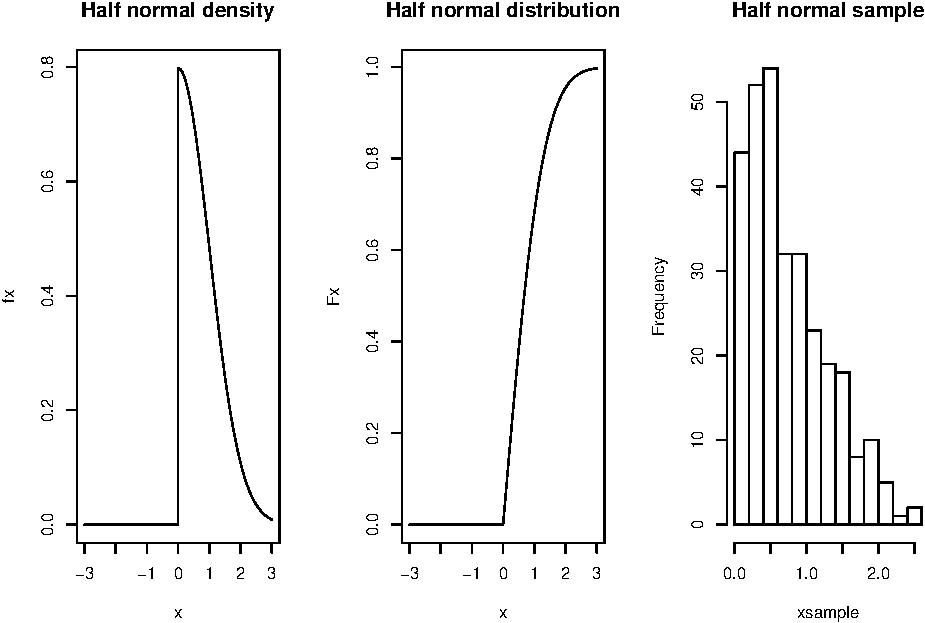
\includegraphics{truncatedDistribution_files/figure-latex/truncated results-1.pdf}

\begin{Shaded}
\begin{Highlighting}[]
         \KeywordTok{par}\NormalTok{(oldPar)}
\end{Highlighting}
\end{Shaded}

\begin{verbatim}
     Hand in the above plots with your code.
          


 c. A 2011 article by Gil Greengross and Geoffrey Miller of the University of New Mexico was entitled "Humor ability reveals intelligence, predicts mating success, and is higher in males" and appeared in Volume 39 of the journal *Intelligence* (pp. 188-192).   
 
     They tested the sense of humour of 400 university students (200 men, 200 women) using a standardized method and found that their measures of humour had about the same standard deviation (0.49) but differed in means with the men scoring an average of 0.09 and the women an average of -0.09 (the higher the score the greater the "humour ability").  The difference in means was found to be statistically significant ($p < 0.001$).
     
     The distributions of humour between men and women seems to be significantly different but what does that actually say?  To get some idea, suppose we take the results to mean that the measure of humour ability for men is $Y \sim N(0.09, (0.49)^2)$ and the same for women is $X \sim N(-0.09, (0.49)^2)$.
     
     i. *(3 marks)* On a single (nicely labelled with a legend) draw the densities (in different colours) for both men and women.
\end{verbatim}

\begin{Shaded}
\begin{Highlighting}[]
\NormalTok{  men <{-}}\StringTok{ }\KeywordTok{rnorm}\NormalTok{(}\DecValTok{200}\NormalTok{, }\DataTypeTok{mean =} \FloatTok{0.09}\NormalTok{, }\DataTypeTok{sd =} \FloatTok{0.49}\NormalTok{)}
\NormalTok{  women <{-}}\StringTok{ }\KeywordTok{rnorm}\NormalTok{(}\DecValTok{200}\NormalTok{, }\DataTypeTok{mean =} \FloatTok{{-}0.09}\NormalTok{, }\DataTypeTok{sd =} \FloatTok{0.49}\NormalTok{)}
\NormalTok{  density\_men =}\StringTok{ }\KeywordTok{density}\NormalTok{(men)}
\NormalTok{  density\_women =}\StringTok{ }\KeywordTok{density}\NormalTok{(women)}
  \KeywordTok{plot}\NormalTok{(density\_men, }\DataTypeTok{col =} \StringTok{"gold"}\NormalTok{, }\DataTypeTok{xlab =} \StringTok{\textquotesingle{}x\textquotesingle{}}\NormalTok{, }\DataTypeTok{main =} \StringTok{"Densities for men and women"}\NormalTok{)}
  \KeywordTok{lines}\NormalTok{(density\_women, }\DataTypeTok{col =} \StringTok{"maroon"}\NormalTok{)}
\KeywordTok{legend}\NormalTok{(}\StringTok{"topright"}\NormalTok{, }\DataTypeTok{legend =} \KeywordTok{c}\NormalTok{(}\StringTok{"men"}\NormalTok{, }\StringTok{"women"}\NormalTok{), }\DataTypeTok{col =} \KeywordTok{c}\NormalTok{(}\StringTok{"gold"}\NormalTok{, }\StringTok{"maroon"}\NormalTok{), }\DataTypeTok{lwd =} \KeywordTok{c}\NormalTok{(}\DecValTok{1}\NormalTok{,}\DecValTok{1}\NormalTok{))}
\end{Highlighting}
\end{Shaded}

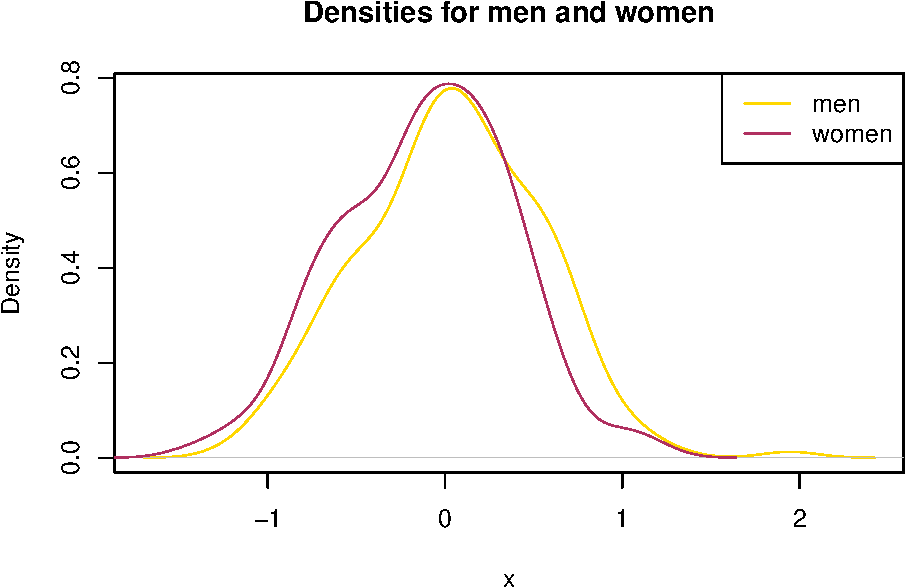
\includegraphics{truncatedDistribution_files/figure-latex/unnamed-chunk-1-1.pdf}

\begin{verbatim}
     ii. *(4 marks)* Generate a random sample of 1000 scores from each of these distributions and save the values on `x` for women, `y` for men, and `results <- data.frame(women = x, men = y)`.  We now have paired results as if in each row, we randomly drew one women and one man and measured their "humour ability".
     
         Based on your sample, estimate the following
         
         - the average humour ability of the men
         - the average humour ability of the women
         - the probability that the man will be funnier than the woman (at least as measured by this scale).
\end{verbatim}

\begin{Shaded}
\begin{Highlighting}[]
\NormalTok{x =}\StringTok{ }\KeywordTok{rnorm}\NormalTok{(}\DecValTok{1000}\NormalTok{, }\DataTypeTok{mean =} \FloatTok{{-}0.09}\NormalTok{, }\DataTypeTok{sd =} \FloatTok{0.49}\NormalTok{)}
\NormalTok{y =}\StringTok{ }\KeywordTok{rnorm}\NormalTok{(}\DecValTok{1000}\NormalTok{, }\DataTypeTok{mean =} \FloatTok{0.09}\NormalTok{, }\DataTypeTok{sd =}\FloatTok{0.49}\NormalTok{)}
\NormalTok{results <{-}}\StringTok{ }\KeywordTok{data.frame}\NormalTok{(}\DataTypeTok{women =}\NormalTok{ x, }\DataTypeTok{men =}\NormalTok{ y)}

\KeywordTok{print}\NormalTok{(}\StringTok{"{-} the average humour ability of the men"}\NormalTok{)}
\end{Highlighting}
\end{Shaded}

\begin{verbatim}
## [1] "- the average humour ability of the men"
\end{verbatim}

\begin{Shaded}
\begin{Highlighting}[]
\KeywordTok{print}\NormalTok{(}\KeywordTok{mean}\NormalTok{(men))}
\end{Highlighting}
\end{Shaded}

\begin{verbatim}
## [1] 0.0387097
\end{verbatim}

\begin{Shaded}
\begin{Highlighting}[]
\KeywordTok{print}\NormalTok{(}\StringTok{"{-} the average humour ability of the women"}\NormalTok{)}
\end{Highlighting}
\end{Shaded}

\begin{verbatim}
## [1] "- the average humour ability of the women"
\end{verbatim}

\begin{Shaded}
\begin{Highlighting}[]
\KeywordTok{print}\NormalTok{(}\KeywordTok{mean}\NormalTok{(women))}
\end{Highlighting}
\end{Shaded}

\begin{verbatim}
## [1] -0.1060419
\end{verbatim}

\begin{Shaded}
\begin{Highlighting}[]
\KeywordTok{print}\NormalTok{(}\StringTok{\textquotesingle{}{-} the probability that the man will be funnier than the woman (at least as measured by this scale)\textquotesingle{}}\NormalTok{)}
\end{Highlighting}
\end{Shaded}

\begin{verbatim}
## [1] "- the probability that the man will be funnier than the woman (at least as measured by this scale)"
\end{verbatim}

\begin{Shaded}
\begin{Highlighting}[]
\CommentTok{\# count one by one....}
\NormalTok{counter =}\StringTok{ }\DecValTok{0}
\ControlFlowTok{for}\NormalTok{(i }\ControlFlowTok{in} \DecValTok{1}\OperatorTok{:}\DecValTok{1000}\NormalTok{)\{}
  \ControlFlowTok{if}\NormalTok{(y[i] }\OperatorTok{>}\StringTok{ }\NormalTok{x[i])\{}
\NormalTok{  counter <{-}}\StringTok{ }\NormalTok{counter }\OperatorTok{+}\StringTok{ }\DecValTok{1}
\NormalTok{  \}}
\NormalTok{\}}
\NormalTok{prob <{-}}\StringTok{ }\NormalTok{counter }\OperatorTok{/}\StringTok{ }\DecValTok{1000}
\KeywordTok{print}\NormalTok{(prob)}
\end{Highlighting}
\end{Shaded}

\begin{verbatim}
## [1] 0.61
\end{verbatim}

\begin{verbatim}
     iii. *(4 marks)*  [Are women funny?](https://www.theguardian.com/commentisfree/2014/mar/04/are-women-funny-you-already-know-the-answer) Suppose that to be really funny (e.g. professional standup comedian) requires a humour ability measure of at least 1.07 (two standard deviations past the mean of the males)
          Generate 1000 pseudo random scores `y` from the truncated distribution for men and another 1000 `x` from the truncated distribution for women.  Form the data frame `funny <- data.frame(women = x, men = y)` and based on this paired sample, estimate the following
         
             - the average humour ability of the men
             - the average humour ability of the women
             - the probability that the man will be funnier than the woman (at least as measured by this scale).
             
\end{verbatim}

\begin{Shaded}
\begin{Highlighting}[]
\NormalTok{      funny <{-}}\StringTok{ }\KeywordTok{truncate}\NormalTok{(}\DataTypeTok{a =} \FloatTok{1.07}\NormalTok{)}
\NormalTok{      men <{-}}\StringTok{ }\NormalTok{funny}\OperatorTok{$}\KeywordTok{rdist}\NormalTok{(}\DecValTok{1000}\NormalTok{, }\DataTypeTok{mean =} \FloatTok{0.09}\NormalTok{, }\DataTypeTok{sd =} \FloatTok{0.49}\NormalTok{) }\CommentTok{\#men}
\NormalTok{      women <{-}}\StringTok{ }\NormalTok{funny}\OperatorTok{$}\KeywordTok{rdist}\NormalTok{(}\DecValTok{1000}\NormalTok{, }\DataTypeTok{mean =} \FloatTok{{-}0.09}\NormalTok{,}\DataTypeTok{sd =} \FloatTok{0.49}\NormalTok{) }\CommentTok{\#women=}
\NormalTok{      res <{-}}\StringTok{ }\KeywordTok{data.frame}\NormalTok{(}\DataTypeTok{women =}\NormalTok{ women, }\DataTypeTok{men =}\NormalTok{ men)}
\NormalTok{      mean\_man <{-}}\StringTok{ }\KeywordTok{mean}\NormalTok{(men)}
\NormalTok{      mean\_women <{-}}\StringTok{ }\KeywordTok{mean}\NormalTok{(women)}
\NormalTok{      count <{-}}\StringTok{ }\DecValTok{0}
      \ControlFlowTok{for}\NormalTok{(i }\ControlFlowTok{in} \DecValTok{1}\OperatorTok{:}\DecValTok{1000}\NormalTok{)\{}
        \ControlFlowTok{if}\NormalTok{(men[i] }\OperatorTok{>}\StringTok{ }\NormalTok{women[i])\{}
\NormalTok{        count <{-}}\StringTok{ }\NormalTok{count }\OperatorTok{+}\StringTok{ }\DecValTok{1}
\NormalTok{        \}}
\NormalTok{      \}}
\NormalTok{      prob <{-}}\StringTok{ }\NormalTok{count}\OperatorTok{/}\DecValTok{1000}
      \KeywordTok{print}\NormalTok{(}\StringTok{\textquotesingle{}{-} the average humour ability of the men\textquotesingle{}}\NormalTok{)}
\end{Highlighting}
\end{Shaded}

\begin{verbatim}
## [1] "- the average humour ability of the men"
\end{verbatim}

\begin{Shaded}
\begin{Highlighting}[]
      \KeywordTok{print}\NormalTok{(mean\_man)}
\end{Highlighting}
\end{Shaded}

\begin{verbatim}
## [1] 1.254786
\end{verbatim}

\begin{Shaded}
\begin{Highlighting}[]
      \KeywordTok{print}\NormalTok{(}\StringTok{\textquotesingle{}{-} the average humour ability of the women\textquotesingle{}}\NormalTok{)}
\end{Highlighting}
\end{Shaded}

\begin{verbatim}
## [1] "- the average humour ability of the women"
\end{verbatim}

\begin{Shaded}
\begin{Highlighting}[]
      \KeywordTok{print}\NormalTok{(mean\_women)}
\end{Highlighting}
\end{Shaded}

\begin{verbatim}
## [1] 1.232599
\end{verbatim}

\begin{Shaded}
\begin{Highlighting}[]
      \KeywordTok{print}\NormalTok{(}\StringTok{\textquotesingle{}{-} the probability that the man will be funnier than the woman (at least as measured by this scale).\textquotesingle{}}\NormalTok{)}
\end{Highlighting}
\end{Shaded}

\begin{verbatim}
## [1] "- the probability that the man will be funnier than the woman (at least as measured by this scale)."
\end{verbatim}

\begin{Shaded}
\begin{Highlighting}[]
      \KeywordTok{print}\NormalTok{(prob)}
\end{Highlighting}
\end{Shaded}

\begin{verbatim}
## [1] 0.528
\end{verbatim}

\begin{verbatim}
    iv. *(2 marks)* What conclusions do you draw about the differences between the humour of men and women?
      
      There is no significant difference between the humor of men and women.
    
    v. *(4 marks)* Repeat part iii, again conditioning on considering only individuals with a "humour ability" score of at least 1.07.   Except now, assume that the means of the female and male score distributions are identical at 0.09 **but** that the standard deviation for the men is 10\% larger for than that for the women (0.049).
    
\end{verbatim}

\begin{Shaded}
\begin{Highlighting}[]
\NormalTok{    funny2 <{-}}\StringTok{ }\KeywordTok{truncate}\NormalTok{(}\DataTypeTok{a =} \FloatTok{1.07}\NormalTok{)}
\NormalTok{      men <{-}}\StringTok{ }\NormalTok{funny2}\OperatorTok{$}\KeywordTok{rdist}\NormalTok{(}\DecValTok{1000}\NormalTok{,}\DataTypeTok{mean =} \FloatTok{0.09}\NormalTok{,}\DataTypeTok{sd =} \FloatTok{0.49} \OperatorTok{*}\StringTok{ }\FloatTok{1.1}\NormalTok{) }\CommentTok{\#men}
\NormalTok{      women <{-}}\StringTok{ }\NormalTok{funny2}\OperatorTok{$}\KeywordTok{rdist}\NormalTok{(}\DecValTok{1000}\NormalTok{,}\DataTypeTok{mean =} \FloatTok{0.09}\NormalTok{,}\DataTypeTok{sd =} \FloatTok{0.49}\NormalTok{) }\CommentTok{\#women}
  
\NormalTok{      result <{-}}\StringTok{ }\KeywordTok{data.frame}\NormalTok{(}\DataTypeTok{women =}\NormalTok{ men, }\DataTypeTok{men =}\NormalTok{ men)}
  
\NormalTok{      mean\_men <{-}}\StringTok{ }\KeywordTok{mean}\NormalTok{(men)}
\NormalTok{      mean\_women <{-}}\StringTok{ }\KeywordTok{mean}\NormalTok{(women)}
\NormalTok{      count <{-}}\StringTok{ }\DecValTok{0}
\NormalTok{      count <{-}}\StringTok{ }\DecValTok{0}
      \ControlFlowTok{for}\NormalTok{(i }\ControlFlowTok{in} \DecValTok{1}\OperatorTok{:}\DecValTok{1000}\NormalTok{)\{}
        \ControlFlowTok{if}\NormalTok{(men[i] }\OperatorTok{>}\StringTok{ }\NormalTok{women[i])\{}
\NormalTok{        count <{-}}\StringTok{ }\NormalTok{count }\OperatorTok{+}\StringTok{ }\DecValTok{1}
\NormalTok{        \}}
\NormalTok{      \}}
\NormalTok{      prob <{-}}\StringTok{ }\NormalTok{count}\OperatorTok{/}\DecValTok{1000}
      \KeywordTok{print}\NormalTok{(}\StringTok{\textquotesingle{}{-} the average humour ability of the men\textquotesingle{}}\NormalTok{)}
\end{Highlighting}
\end{Shaded}

\begin{verbatim}
## [1] "- the average humour ability of the men"
\end{verbatim}

\begin{Shaded}
\begin{Highlighting}[]
      \KeywordTok{print}\NormalTok{(mean\_man)}
\end{Highlighting}
\end{Shaded}

\begin{verbatim}
## [1] 1.254786
\end{verbatim}

\begin{Shaded}
\begin{Highlighting}[]
      \KeywordTok{print}\NormalTok{(}\StringTok{\textquotesingle{}{-} the average humour ability of the women\textquotesingle{}}\NormalTok{)}
\end{Highlighting}
\end{Shaded}

\begin{verbatim}
## [1] "- the average humour ability of the women"
\end{verbatim}

\begin{Shaded}
\begin{Highlighting}[]
      \KeywordTok{print}\NormalTok{(mean\_women)}
\end{Highlighting}
\end{Shaded}

\begin{verbatim}
## [1] 1.253287
\end{verbatim}

\begin{Shaded}
\begin{Highlighting}[]
      \KeywordTok{print}\NormalTok{(}\StringTok{\textquotesingle{}{-} the probability that the man will be funnier than the woman (at least as measured by this scale).\textquotesingle{}}\NormalTok{)}
\end{Highlighting}
\end{Shaded}

\begin{verbatim}
## [1] "- the probability that the man will be funnier than the woman (at least as measured by this scale)."
\end{verbatim}

\begin{Shaded}
\begin{Highlighting}[]
      \KeywordTok{print}\NormalTok{(prob)}
\end{Highlighting}
\end{Shaded}

\begin{verbatim}
## [1] 0.56
\end{verbatim}

\end{document}
